\documentclass[10pt]{beamer}

\usetheme[progressbar=frametitle]{metropolis}
\usepackage{appendixnumberbeamer}

\usepackage{booktabs}
\usepackage[scale=2]{ccicons}

\usepackage{pgfplots}
\usepgfplotslibrary{dateplot}

\usepackage{xspace}
\newcommand{\themename}{\textbf{\textsc{metropolis}}\xspace}

% \usepackage{enumitem}

\metroset{titleformat frame=smallcaps}

% \setbeamercolor*{structure}{bg=Red!20,fg=Red}

% \setbeamercolor*{palette primary}{use=structure,fg=white,bg=structure.fg}
% \setbeamercolor*{palette secondary}{use=structure,fg=white,bg=structure.fg!75}
% \setbeamercolor*{palette tertiary}{use=structure,fg=white,bg=structure.fg!50!black}
% \setbeamercolor*{palette quaternary}{fg=white,bg=black}

% \setbeamercolor{section in toc}{fg=black,bg=white}
% \setbeamercolor{alerted text}{use=structure,fg=structure.fg!50!black!80!black}

% \setbeamercolor{titlelike}{parent=palette primary,fg=structure.fg!50!black}
% \setbeamercolor{frametitle}{bg=gray!10!white,fg=PineGreen}

% \setbeamercolor*{titlelike}{parent=palette primary}

\usepackage[
backend=biber,
style=authortitle,
]{biblatex}
\addbibresource{editing-embedding.bib} % Import bibliography file
\let\svthefootnote\thefootnote
\textheight 1in
\newcommand\blankfootnote[1]{%
  \let\thefootnote\relax\footnotetext{#1}%
  \let\thefootnote\svthefootnote%
}
\let\svfootnote\footnote
\renewcommand\footnote[2][?]{%
  \if\relax#1\relax%
    \blankfootnote{#2}%
  \else%
    \if?#1\svfootnote{#2}\else\svfootnote[#1]{#2}\fi%
  \fi
}
\title{Editing in Embedding Space}
% \subtitle{A modern beamer theme}
% \date{\today}
\date{}
\author{Me}
% \institute{}
% \titlegraphic{\hfill\includegraphics[height=1.5cm]{logo.pdf}}

\begin{document}

\maketitle

\section{Part 1}
\begin{frame}{Classic Arithmetic}

\begin{center}
    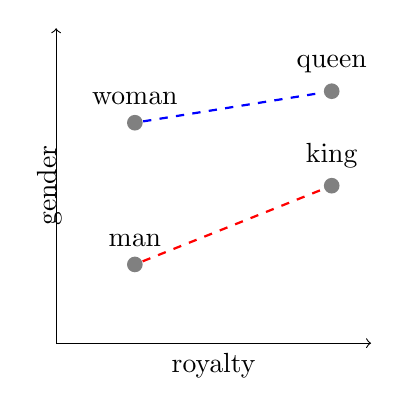
\begin{tikzpicture}
        % styles
        \tikzstyle{word}=[circle, fill=gray, inner sep=2pt]
        \tikzstyle{vector}=[dashed, -, >=stealth, thick]
        
        % axes
        \draw[->] (0,0) -- (4,0) node[midway,below] {royalty};
        \draw[->] (0,0) -- (0,4) node[midway, left, rotate=90, anchor=base] {gender};
        
        % words
        \node[word, label={above:man}] (man) at (1,1) {};
        \node[word, label={above:king}] (king) at (3.5,2) {};
        \node[word, label={above:woman}] (woman) at (1,2.8) {};
        \node[word, label={above:queen}] (queen) at (3.5,3.2) {};
        
        % vectors
        \draw[vector, red] (man) -- (king) node[midway, above, sloped] {};
        \draw[vector, blue] (woman) -- (queen) node[midway, above, sloped] {};
    \end{tikzpicture}
\end{center}
\begin{align*}
    \overrightarrow{\text{king}} - \overrightarrow{\text{man}} + \overrightarrow{\text{woman}}
    &\approx \overrightarrow{\text{queen}}\\
    \overrightarrow{\text{man}} - \overrightarrow{\text{woman}} &\approx \overrightarrow{\text{king}} - \overrightarrow{\text{queen}}
\end{align*}
\end{frame}

\begin{frame}{Analogy Discovery \& Bias}
\begin{figure}[t]
\centering
    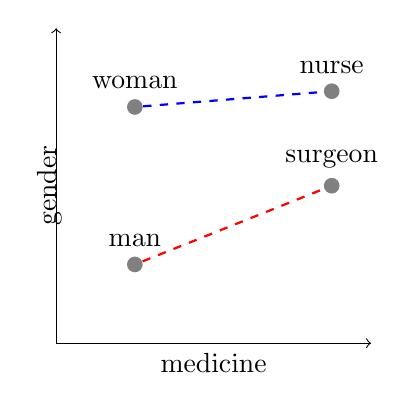
\begin{tikzpicture}
        % styles
        \tikzstyle{word}=[circle, fill=gray, inner sep=2pt]
        \tikzstyle{vector}=[dashed, -, >=stealth, thick]
        
        % axes
        \draw[->] (0,0) -- (4,0) node[midway,below] {medicine};
        \draw[->] (0,0) -- (0,4) node[midway, left, rotate=90, anchor=base] {gender};
        
        % words
        \node[word, label={above:man}] (man) at (1,1) {};
        \node[word, label={above:surgeon}] (surgeon) at (3.5,2) {};
        \node[word, label={above:woman}] (woman) at (1,3) {};
        \node[word, label={above:nurse}] (nurse) at (3.5,3.2) {};
        
        % vectors
        \draw[vector, red] (man) -- (surgeon) node[midway, above, sloped] {};
        \draw[vector, blue] (woman) -- (nurse) node[midway, above, sloped] {};
    \end{tikzpicture}
    \caption{Cartoon of (real) biased analogy in embedding space.}
    % \label{fig:something}
\end{figure}

\blankfootnote{\cite{bolukbasi2016man}}
\end{frame}

\begin{frame}{Debiasing Embeddings}
How do we edit embeddings and maintain utility?\footnote{\cite{bolukbasi2016man}} (e.g. reduce gender bias with minimal residual impact)
\begin{enumerate}
    \item<1-> Identify a target subspace
    \only<2>{
            \metroset{block=fill}
            \begin{block}{Subspace}
                Recall a subspace is an inner product/vector space,
                \begin{enumerate}
                    \item[1.] Conjugate symmetry: $\langle x, y\rangle = \overline{\langle y, x\rangle}$
                    \item[2.] Linearity: $\langle ax + by, z\rangle = a\langle x, z\rangle + b\langle y, z\rangle$
                    \item[3.] Positive-definiteness: $\langle x, x\rangle > 0$ if $x \neq 0$
                \end{enumerate}
            \end{block}
    }
    \item<3-> Edit embeddings by either
    \begin{enumerate}
        \item<3-> Deleting the subspace
        \item<3-> Soft transformation (e.g. shear)
    \end{enumerate}
\end{enumerate}
\only<4>{
Option 1 prioritizes removal.\\
Option 2 attempts to balance removal with utility preservation,
\[
\min_T  \| (TW)^T(TW)-W^T W \|_F^2 + \lambda \|(TN)^T(TB)\|_F^2.
\]}
 % Let $X = T^T T$, then this is equivalent to the following semi-definite programming problem
% \begin{equation}
% \label{eq:sdp}
% \min_X \| W^T X W - W^T W \|_F^2 + \lambda \| N^T X B\|_F^2 \qquad \mbox{s.t.}  X\succeq 0.
% \end{equation}
% The first term ensures that the pairwise inner products are preserved and the second term induces the biases of gender neutral words onto the gender subspace to be small. The user-specified parameter $\lambda$ balances the two terms.
% \[
% \min_T  \| (TW)^T(TW)-W^T W \|_F^2 + \lambda \|(TN)^T(TB)\|_F^2.
% \]
\only<5>{Can we do better? \footnote{\cite{gonen-goldberg-2019-lipstick}}}
\end{frame}

\begin{frame}{Iterative Nullspace Projection}
What if we did not have to presuppose a direction and could learn one instead?
\begin{itemize}
    \item Learn a classifier
    \pause
    \item Project onto nullspace
    \pause
    \item Repeat
\end{itemize}
\pause
Math aside, this is an intuitive approach:
\begin{enumerate}
    \item Try to separate the data
    \pause
    \item Is the data linearly separable?
    \pause
    \item Yes? Make it less separable. No? Done.
\end{enumerate}
\blankfootnote{\cite{ravfogel-etal-2020-null}}
\end{frame}

\begin{frame}{Iterative Nullspace Projection}
    \begin{figure}[t]
        \centering
        \includegraphics[width=0.8\columnwidth]{assets/nullspace-projection.png}
        
        % \includegraphics[width=\linewidth]{plots/nullspace-projection.png}
        \caption{For binary classifier along $W$ the decision boundary is formed by $N(W)$, onto which we can project points.}
        \label{fig:nullspace-projection}
    \end{figure} 
\blankfootnote{\cite{ravfogel-etal-2020-null}}
\end{frame}

\section{
Part II (Next time)
}

\begin{frame}{Adversarial Concept Erasure}

\begin{figure}[t]
    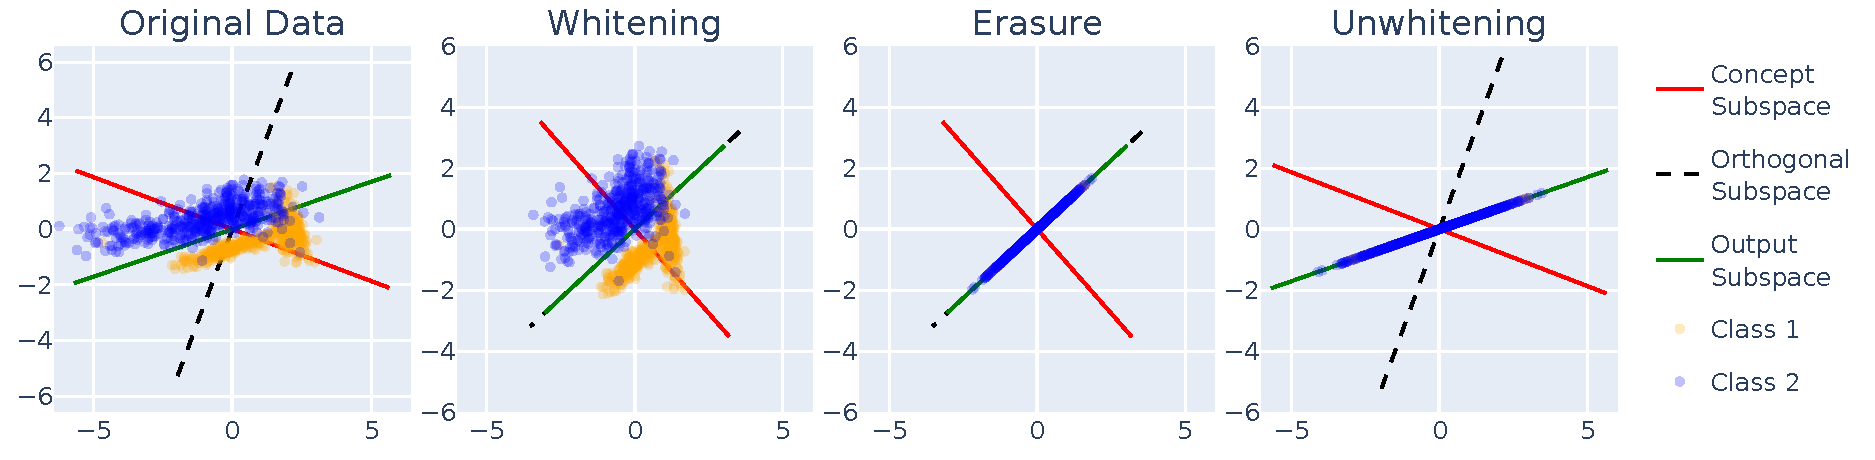
\includegraphics[width=0.6\columnwidth]{assets/leace-process.pdf}
    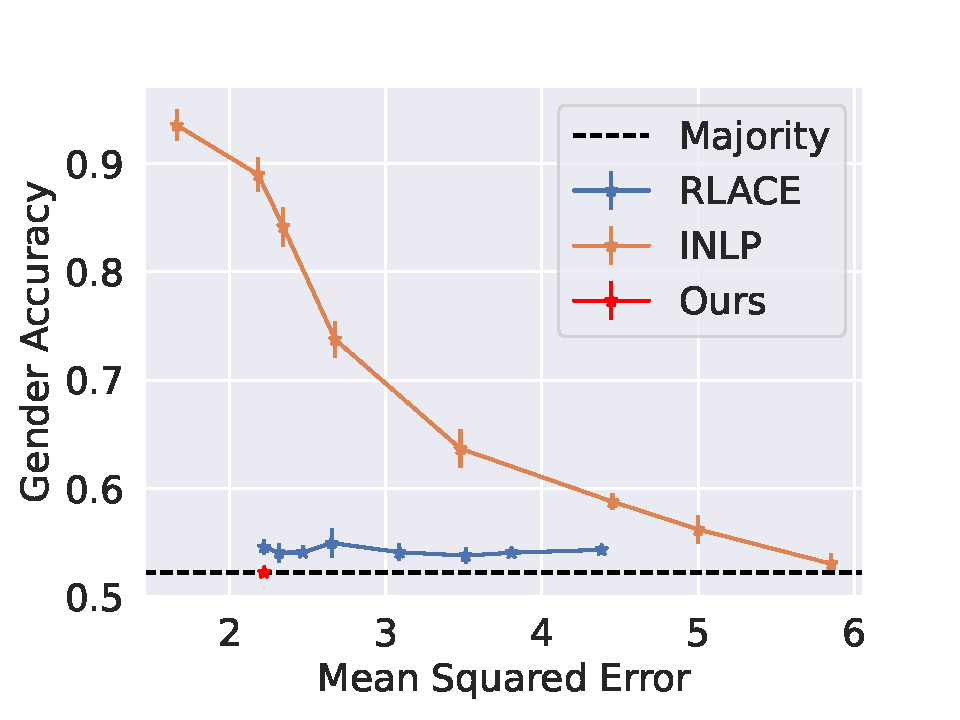
\includegraphics[width=0.5\columnwidth]{assets/lease-lace-inlp-acc-vs-mse.pdf}
\end{figure} 

\cite{pmlr-v162-ravfogel22a}

\cite{belrose2023leaceperfectlinearconcept}
\end{frame}

\appendix

% \begin{frame}[fragile]{Backup slides}
%   Sometimes, it is useful to add slides at the end of your presentation to
%   refer to during audience questions.

%   The best way to do this is to include the \verb|appendixnumberbeamer|
%   package in your preamble and call \verb|\appendix| before your backup slides.

%   \themename will automatically turn off slide numbering and progress bars for
%   slides in the appendix.
% \end{frame}
% \begin{frame}[allowframebreaks]{References}

%   % \bibliography{editing-embedding}
%   % \bibliographystyle{abbrv}

% \end{frame}

\end{document}
